% Options for packages loaded elsewhere
\PassOptionsToPackage{unicode}{hyperref}
\PassOptionsToPackage{hyphens}{url}

%
\documentclass[ignorenonframetext,fleqn]{beamer}
% \usepackage{showframe}
% ---------------------------------------------------------------%
\usetheme[]{Copenhagen}
\useoutertheme{infolines}
\setbeamertemplate{navigation symbols}{}

\usepackage[backend=biber, style=authoryear, natbib=true]{biblatex}
\addbibresource{references.bib}

\usepackage{bibentry}
\usepackage{subcaption}
\usepackage{graphicx}
\usepackage{pgfpages}
\usepackage{soul}
% Prevent slide breaks in the middle of a paragraph
\usepackage{amsmath,amssymb,amsfonts}
% Use upquote if available, for straight quotes in verbatim environments
\IfFileExists{upquote.sty}{\usepackage{upquote}}{}
\providecommand{\tightlist}{%
  \setlength{\itemsep}{0pt}\setlength{\parskip}{0pt}}
\setcounter{secnumdepth}{-\maxdimen} % remove section numbering
\usepackage{tikz-cd}
\usepackage{adjustbox}

\usepackage{tikz}
\usetikzlibrary{arrows.meta, positioning, decorations.pathmorphing}

\title{Equivalence in Foundations}
\author{Laney Gold-Rappe and Hans Halvorson}
\date{June 28, 2024}

%% TO DO: Mitchell-Benabou language

%% TO DO: cite papers by Evan Washington, and Visser's student 

\newcommand{\2}{\mathcal}

\usepackage{pifont}
\usepackage{xcolor}

\newcommand{\cmark}{\textcolor{green}{\ding{51}}} % Check mark
\newcommand{\xmark}{\textcolor{red}{\ding{55}}}   % X mark

\begin{document}
\frame{\titlepage}



\begin{frame}{The old consensus}

  \begin{itemize}
  \item Early 20th century: Zermelo-Frankel set theory won the battle
    about the foundations of mathematics.
  \item Defeated competitors:
    \begin{itemize}
    \item Logicism
    \item Finitism
    \item Intuitionism
    \item Type theory
    \end{itemize}
  \item Philosophers take set theory as background framework for their
    inquiries. \newline {\footnotesize See: \fullcite{lewis-worlds}}
  \end{itemize}

\end{frame}


\begin{frame}{New developments}

  \begin{itemize}
  \item Category theory and topos theory have proved fruitful in
    various branches of pure mathematics (Grothendieck, Mac Lane,
    Lawvere)
  \item Martin-L{\"o}f type theory
  \item Computation
  \item Homotopy type theory (HoTT)
  \item Philosophical worries about set theory (structuralism, etc.)
  \end{itemize}

\end{frame}

\begin{frame}{Motivation}

  What got me (HH) worried about set-theoretic foundations is that it
  seems to have too much ``sand'' for use in the foundations of
  physics.

  \bigskip Isomorphic models can have different features qua sets:
  \begin{itemize}
  \item $M\vDash \phi (a)$ but $N\vDash \neg \phi (a)$.
  \item $\{ \emptyset \}\in M$ but $\{ \emptyset \}\not\in N$.
  \end{itemize}

\end{frame}

\begin{frame}{Motivation}

  \begin{itemize}
  \item It would seem natural to replace ZF with an elementary topos
    $\2E$, thereby ignoring the (otiose?) universal membership
    relation.
  \item In a topos, $x=y$ has no meaning for $x:A$ and $y:B$, with
    $A\neq B$.
  \item Question: Can isomorphic $\2E$-models of $T$ have different
    properties? It's important to be clear here about what ``different
    properties'' means.
  \end{itemize}  

\end{frame}

\begin{frame}{Motivation}

  \begin{itemize}
  \item Topos-theoretic foundations are (apparently) more
    general. E.g.\ the axioms of synthetic differential geometry have
    no model in Sets, but do have a model in a topos.
  \end{itemize}

\end{frame}


\begin{frame}{Is a new battle coming?}

\begin{itemize}  
\item Feferman \citeyearpar{feferman1969,feferman1977} argues against
  category-theoretic foundations for philosophical reasons: the idea
  of ``aggregating'' is presupposed even in category theory.
\item The idea that Sets and Cats are incommensurable foundations was
  challenged via results of Mitchell, Osius, and Mathias
  \begin{itemize}
  \item What exactly did they prove?
  \end{itemize}
\end{itemize}

\end{frame}

\begin{frame}{Goals of this project}

  \begin{itemize}
  \item Evaluate Awodey's \citeyearpar{awodey} claim that Sets, Cats,
    and Types are equivalent foundations.\footnote{\citet{linnebo}
      also suggest that Sets and Types are equivalent foundations, but
      don't suggest any kind of formal proof.}
  \item Evaluate whether \citet{shulman} has established that ZFC and
    ETCS+R are bi-interpretable.
  \item Sharpen the definition of bi-interpretability and compare it
    to other notions of equivalence.
  \end{itemize}

\end{frame}

\begin{frame}{What do we mean by equivalent?}

\scalebox{0.7}{
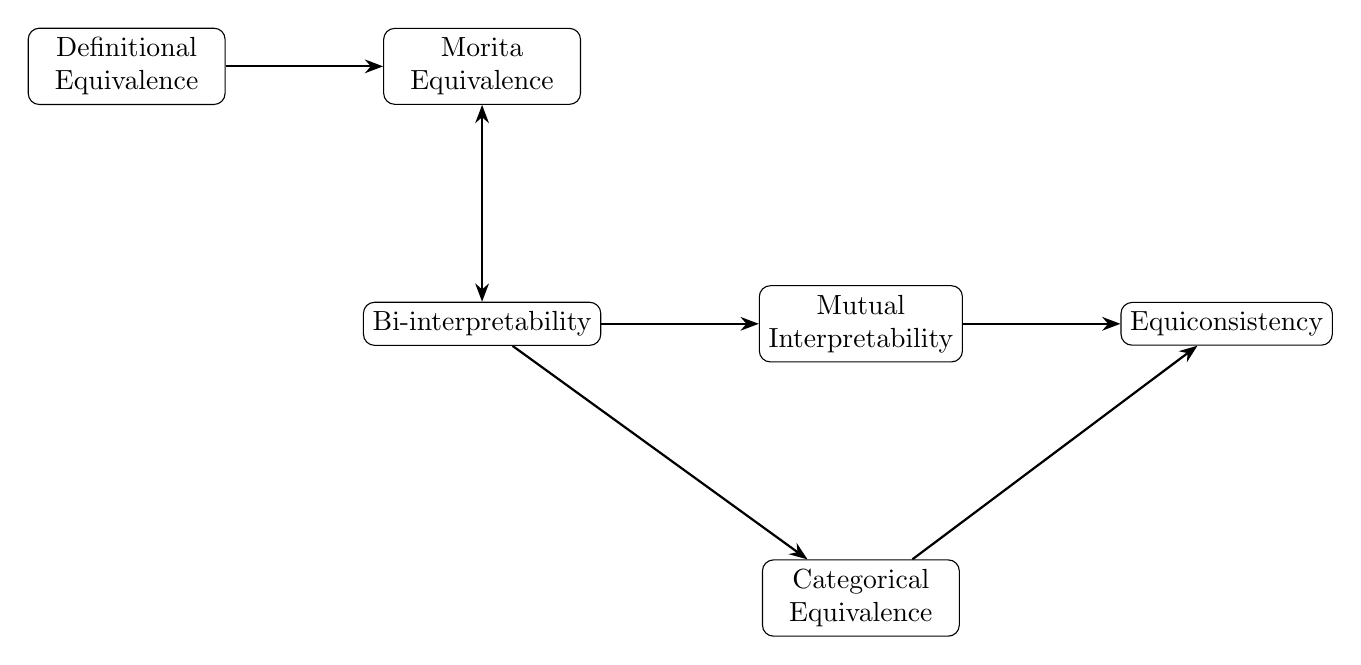
\begin{tikzpicture}[
  node distance=2.5cm and 2cm,
  every node/.style={draw, rectangle, rounded corners, minimum height=1.5em, minimum width=2.5cm, align=center},
  arrow/.style={-Stealth, thick},
  doublearrow/.style={Stealth-Stealth, thick}
]

% Nodes for the first row
\node (definitional) {Definitional \\ Equivalence};
\node (morita) [right=of definitional] {Morita \\ Equivalence};

% Nodes for the second row
\node (bi) [below=of morita, node distance=2cm] {Bi-interpretability};
\node (mutual) [right=of bi] {Mutual \\ Interpretability};
\node (equi) [right=of mutual] {Equiconsistency};

% Nodes for the third row
\node (cat) [below=of mutual] {Categorical \\ Equivalence};

% Arrows for logical implications
\draw[arrow] (definitional) -- (morita);
\draw[arrow] (bi) -- (mutual);
\draw[arrow] (mutual) -- (equi);
\draw[arrow] (bi) -- (cat);
\draw[arrow] (cat) -- (equi);

% Vertical double arrows for logical equivalence
\draw[doublearrow] (morita) -- (bi);

\end{tikzpicture} }

  \nocite{maclane} \nocite{mclarty2004}


\end{frame}

\begin{frame}{Equivalence and syntactic categories}

  \begin{itemize}
  \item Morita equivalence \citep{morita} is an attempt to give an
    elementary expression of the idea that $\mathrm{Sh}(C_T)$ and
    $\mathrm{Sh}(C_{T'})$ are equivalent toposes
    \citep[see][]{makkai2006}.
  \item Morita equivalence is very likely (perhaps some fine-tuning
    needed?) the same thing as bi-interpretability
    \citep[see][]{halvorson}.
  \item Note: Morita equivalence is weaker (more liberal) than the
    notion that $C_T$ and $C_{T'}$ are equivalent categories.
   \end{itemize} 

\end{frame}

\begin{frame}{Why bi-interpretability matters}

  \nocite{friedman2014bi} \nocite{freire}

  \textbf{Informal Hypothesis:} \textit{Bi-interpretability ensures
    that the theories share all relevant properties.}

  \vfill \begin{itemize}
  \item Fact: Mutual interpretability does not imply
    bi-interpretability.
    \begin{itemize}
    \item ZF and ZFC are mutually interpretable, but not
      bi-interpretable (see Enayat).
    \item \fullcite{andreka}
    \end{itemize}  
  \item To do: Examples of mutually interpretable theories that have
    different properties (model-theoretic, proof-theoretic, etc.)
  \end{itemize}

\end{frame}

\begin{frame}{Properties preserved under equivalence}

  %% is the spectrum of a theory preserved under bi-interpretability? 

  \begin{center}
  \begin{tabular}{l|c|c}
    & mutual int & bi-int \\ \hline
    $\kappa$-categorical & & \cmark \\ \hline 
    finitely axiomatizable & & \cmark \\ \hline
    model complete & & \cmark \\ \hline
    $\omega$-stable & & \\ \hline 
    has a prime model & & \\ \hline 
    strongly minimal & & 
  \end{tabular}
  \end{center}



\end{frame}

\begin{frame}{Why bi-interpretability matters}

  \textbf{Informal Hypothesis:} \textit{Bi-interpretability is our
    best account of expressive equivalence.}

  \vfill For each $\Sigma _1$-formula $\phi$, there is a
  $\Sigma _2$-formula $F(\phi )$ that ``says the same thing''.

\end{frame}


\begin{frame}{Bi-interpretability: syntax and semantics}

  \begin{center}
    \begin{tikzpicture}
    % Nodes on first row
    \node (ETCS) at (0, 4) {ETCS};
    \node (ZF) at (4, 4) {ZF};

    % Nodes on second row 
    \node (Set) at (0, 0) {$\2E$};
    \node (V) at (4, 0) {$U$};

     % Curved Arrows
    \draw[->, bend left=30] (ETCS) to (ZF);
    \draw[->, bend left=30] (ZF) to (ETCS);
        
    % Optional: arrows from top to bottom
    %\draw[->] (ETCS) -- (Set);
    %\draw[->] (ZF) -- (V);
  \end{tikzpicture}
  \end{center}

\end{frame}

\begin{frame}{Translation}

  The notion of \textbf{translation} is still a work in
  progress\footnote{The first explicit definition of a translation
    with arity $n\geq 1$ seems to be \citep{szczerba}. The idea is
    developed further in \citep{benthem,visser2006}. For an attempt to
    systematize, see \citep{halvorson}.} --- although it seems to be
  implicit in much of the standard literature.

  \begin{itemize}
  \item A translation $F$ has an arity $n_F$, which says how many
    variables to split a single variable into.
  \item A translation $F$ has a domain formulas $\delta ^F_\sigma$ in
    the target language.
  \item A translation represents equality $=$ in $\Sigma$ in terms of
    some $T'$-provable equivalence relation in $\Sigma '$.
  \end{itemize}



\end{frame}


\begin{frame}{$2$-cells between translations}

 \begin{center}
  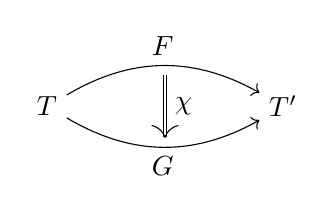
\begin{tikzpicture}
  \node (A) at (0,0) {$T$};
  \node (B) at (3,0) {$T'$};

  \draw[->] (A) to[bend left=30] node[above] {$F$} (B);
  \draw[->] (A) to[bend right=30] node[below] {$G$} (B);

  \draw[->, double] (1.5,0.4) -- (1.5,-0.4) node[midway, right] {$\chi$};
\end{tikzpicture}
\end{center}

Roughly speaking: A $2$-cell $\chi :F\Rightarrow G$ is a formula in
$\Sigma '$ that represents a functional relation from the domain
formula of $F$ to the domain formula of $G$ and that maps the
extension of $F(R)$ to the extension of $G(R)$, for each relation
symbol $R$ of $\Sigma$.\footnote{This idea is implicit throughout
  model theory, and is more explicit in \citep{visser2006}.}

\end{frame}

\begin{frame}

  \begin{block}{Definition} Let $F:T\to T'$ and $G:T'\to T$ be
    translations. We say that $F$ and $G$ form an \textbf{equivalence}
    just in case there are invertible 2-cells
    $\eta :1_T\Rightarrow GF$ and $\varepsilon :1_{T'}\Rightarrow FG$.
  \end{block}  



\end{frame}

\begin{frame}

  A translation $F:T\to T'$ determines a functor
  $F^*:\mathrm{Mod}(T')\to\mathrm{Mod}(T)$. See
  \citep{gajda,halvorson}

  \vfill In particular, $F^*(M)$ is $n_F$ copies of $D(M)$, quotiented
  by the equivalence relation $=_F$.
  
\end{frame}

\begin{frame}

  To be checked: a 2-cell $\chi :F\Rightarrow G$ should determine a
  natural transformation $\chi ^*:F^*\Rightarrow G^*$.

  \bigskip Note: $\chi ^*$ is not just any natural transformation, but
  is induced uniformly via a $\Sigma '$-formula that is a
  $T'$-provable functional relation.

\end{frame}


\begin{frame}{Proving equivalence semantically}

  Given functors $f:\mathrm{Mod}(T')\to\mathrm{Mod}(T)$ and
  $g:\mathrm{Mod}(T)\to\mathrm{Mod}(T')$, under what conditions on $f$
  and $g$ establish that $T$ and $T'$ are bi-interpretable?

  \vfill See \citep{gajda}



\end{frame}

\begin{frame}

  What are the natural isomorphisms on the two sides? 

  If ZF and ETCS are bi-interpretable, then there are linking formulas 
  



\end{frame}

\begin{frame}{Topos-theoretic foundations of mathematics}

  \begin{block}{Definition}
    An \textbf{elementary topos} $\2E$ is a category that has the
    following properties:
        \begin{itemize}
        \item Finite limits.
        \item Exponentials: For any objects $A, B \in \mathcal{E}$,
          there exists an object $B^A$ and an evaluation map
          $ev: B^A \times A \to B$ such that for any object $C$ and
          any map $f: C \times A \to B$, there is a unique map
          $\lambda f: C \to B^A$ making the appropriate diagram
          commute.
        \item A subobject classifier $\Omega$: An object $\Omega$ with
          a morphism $true: 1 \to \Omega$ such that for any
          monomorphism $m: A \to B$, there exists a unique
          characteristic morphism $\chi_m: B \to \Omega$ making the
          diagram commute.
       \end{itemize}
     \end{block}

\end{frame}

\begin{frame}{Category Axioms}
    \begin{block}{Objects and Morphisms}
        \begin{itemize}
            \item Two sorts: \textbf{Objects} and \textbf{Morphisms}.
            \item Each morphism \( f \) has a \textbf{domain} \( \text{dom}(f) \) and \textbf{codomain} \( \text{cod}(f) \).
        \end{itemize}
    \end{block}
    \begin{block}{Composition}
        \begin{itemize}
            \item For any morphisms \( f \) and \( g \) with \( \text{cod}(f) = \text{dom}(g) \), there is a composite morphism \( g \circ f \).
        \end{itemize}
    \end{block}
    \begin{block}{Associativity}
        \begin{itemize}
            \item For any morphisms \( f, g, h \): $h \circ (g \circ f) = (h \circ g) \circ f$
        \end{itemize}
    \end{block}
    \begin{block}{Identity}
        \begin{itemize}
            \item For each object \( A \), there is an identity morphism \( \text{id}_A \).
            \item For any morphism \( f \): $\text{id}_{\text{dom}(f)}
              \circ f = f \quad \text{and} \quad f \circ
              \text{id}_{\text{cod}(f)} = f $
        \end{itemize}
    \end{block}
  \end{frame}

\begin{frame}{Finite Limits}
    \begin{block}{Terminal Object}
        \begin{itemize}
            \item There is an object \( 1 \) (terminal object) such that for any object \( A \), there is a unique morphism \( !: A \to 1 \).
        \end{itemize}
    \end{block}
    \begin{block}{Pullbacks}
        \begin{itemize}
            \item For any pair of morphisms \( f: A \to C \) and \( g: B \to C \), there exists a pullback square:
   \[
            \begin{tikzcd}[ampersand replacement = \&]
            P \arrow[r] \arrow[d] \& B \arrow[d, "g"] \\
            A \arrow[r, "f"] \& C
            \end{tikzcd}
            \]
        \end{itemize}
    \end{block}
  \end{frame}

\begin{frame}{Topos-theoretic foundations}

  We include in our axioms for topos-theoretic foundations: NNO,
  Boolean, axiom of choice.



\end{frame}
    

\begin{frame}{Topos-theoretic foundations}

\begin{block}{Element}
For an object $A$ in $\2E$, an \textbf{element} of $A$ is an arrow
$x:1\to A$.
\end{block}

    
\end{frame}

\begin{frame}{Intuitive differences between \textbf{Set} and
      \textbf{Cat}}

  In \textbf{Set}: any two sets can stand in the elementhood
  relationship with each other.


\end{frame}


\begin{frame}{The question of framework}

  \begin{itemize}
  \item Since both ZF and ETCS can be formulated in many-sorted,
    classical, first-order logic, they can be compared by standard
    tools (such as bi-interpretability). 
  \item But there is a sense in which ``thinking categorically'' or
    ``thinking type-theoretically'' does not sit well within this
    framework.
  \end{itemize}


\end{frame}  


\begin{frame}{Shulman's Theorem}



  \citet{shulman} seems very close to proving bi-interpretability of
  ZF and ETCS.

  \begin{itemize}
  \item For each model $U$ of ZF, there is a corresponding model of
    ETCS; and for each model $\2E$ of ETCS, there is a corresponding
    model of ZF.
  \item What are the permitted constructions?
  \item In what sense is the construction uniform, i.e.\ doesn't
    depend on specific features of a model?
  \item What needs to be shown about the constructions?
  \end{itemize}


\end{frame}

\begin{frame}{From universe to topos}

  \begin{enumerate}
  \item Given a model $\langle U,\in \rangle$ of ZF, let
    $\mathcal{E}_0=U$, and let $\mathcal{E}_1$ be the set of functions
    between sets (constructed as subsets of ordered pairs).
  \item Fact: the pair $\mathcal{E}_0,\mathcal{E}_1$ forms a model of
    ETCS.
    \begin{itemize}
    \item The empty set is an initial object.
    \item Any singleton set is a terminal object.
    \item Etc.
    \end{itemize}
  \end{enumerate}

\end{frame}

\begin{frame}{From topos to universe}

  \begin{itemize}
  \item Intuitively, the objects in $\2E$ would become sets. But how
    to define the relation $A\in B$?
  \item So instead of taking objects in $\2E$ as sets, we take trees: 
    \[ t:R \rightarrowtail A\times A \]
   \end{itemize}

\end{frame}

\begin{frame}

  For elements $a:1\to A$ and $b:1\to A$, we write $a\leq b$ just in
  case

  \bigskip \begin{tikzcd}[ampersand replacement=\&]
  \& R \arrow[d, "t"] \\
  1 \arrow[ur, dashed, "r"] \arrow[r, "{(a,b)}"'] \& A \times A \arrow[r, shift left, "p_1"] \arrow[r, shift right, "p_2"'] \& A
\end{tikzcd}




\end{frame}

\begin{frame}{Construction of ZF model from ETCS model}

  \includegraphics[scale=0.3]{tree.jpg}


\end{frame}
 

\begin{frame}

   %% When Shulman talks about "every node" I don't understand if he
   %% means literally every "element" of the object A

   \begin{description}
   \item[Tree:] A \textbf{tree} is a poset that is downward linear.
   \item[Rooted:] If $t:R\rightarrowtail A\times A$ is a tree, and
     $e:1\to A$, then we say that $e$ is the \textbf{root} of $t$ just
     in case $\forall x(e\leq x)$.
   \item[Accessible:] A pointed tree $(t,e)$ is \textbf{accessible}
     just in case: for every element $x:1\to A$ there is a finite
     $R$-path to the root $e:1\to A$.\footnote{This definition can be made
     first-order using subobjects of the natural number object in
     $\2E$.}
   \end{description}

\end{frame}

\begin{frame}

  A subobject $m:S\rightarrowtail A$ is said to be \textbf{inductive}
  for the tree $t:R\rightarrowtail A\times A$ just in case: for any
  element $x:1\to A$, if every $y\leq x$ factors through $m$, then $x$
  factors through $m$.


\end{frame}
 

 \begin{frame}

   \begin{description}
   \item[Well-founded:] If $m:S\rightarrowtail X$ is inductive, then
     $m$ is an isomorphism.
   \item[Extensional:] For any $x:1\to A$ and $y:1\to A$, if $x$ and
     $y$ have the same $R$-children, then $x=y$.
     %% is equality needed here, or just isomorphism? 
   \end{description}

 \end{frame}
  

\begin{frame}

  How do we know that there are ``enough'' of these trees in $\2E$ to
  build an entire ZF universe?


\end{frame}

\begin{frame}{Questions about Shulman's result}

  \begin{itemize}
  \item The construction of trees from a topos $\2E$ seems to require
    infinitary procedures. Is this move permitted by the standard
    definition of bi-interpretability?
  \end{itemize}


\end{frame}

\begin{frame}{A simple example}

  $T_1$ says that there are exactly two things.

  $T_2$ says that there are exactly two atoms, and one mereological
  sum of those atoms.

  
  



\end{frame}



\begin{frame}

  To establish bi-interpretability, it needs to be shown that there is
  a formula $\chi$ (in the language of category theory) that defines
  an isomorphism between $GF(\2E )$ and $\2E$.


\end{frame}

\begin{frame}{Type theory: Kemeny or Awodey?}

  ``It was my intention to prove the equivalence of the simple theory
  of types and Zermelo set-theory. Instead of this I have succeeded in
  proving a strong theorem from which it follows that the two systems
  are not equivalent under \underline{any} reasonable definition of
  `equivalent'.'' \citep{kemeny}

  \nocite{mathias} \nocite{pinter}


\end{frame}

\begin{frame}{Questions and Conjectures}

  Is the following an example of mutually interpretable theories that
  are not bi-interpretable?

\bigskip $T_1$ is the theory of a field with $2$ elements.

$T_2$ is the theory of fields of characteristic $2$.

\bigskip It depends on what we mean by ``bi-interpretable''. If
equality has to be translated strictly, then there is no translation
from $T_1$ to $T_2$.

%% claimed by Carl Mummert on
%% https://math.stackexchange.com/questions/621932/do-metatheoretic-results-carry-between-mutually-interpretable-theories

\end{frame}

\begin{frame}{Questions and Conjectures}

  K. Williams argues that bi-interpretability is not strong enough: 
  \url{http://kamerynjw.net/2022/05/18/bi-interpretability.html}

\end{frame}

\begin{frame}{Questions and Conjectures}

  \begin{itemize}
  \item Dependent type theory is a more natural setting for theory of
    categories and the elementary theory of toposes.
    \begin{itemize}
    \item Replace ``isomorphism'' with ``equivalence''.
    \end{itemize}
  \item If ETCS and ZF are formalized in FOLDS \citep{makkai}, does
    the equivalence result still hold?
  \end{itemize}

\end{frame}

\begin{frame}{Questions and Conjectures}

  \begin{itemize}
  \item Does the category $\underline{\mathrm{hom}}(T,T')$ of
    translations from $T$ to $T'$ correspond to a certain category of
    functors between the syntactic categories $C_T$ and $C_{T'}$?
  \item It's tempting to move to a purely categorical framework (e.g.\
    replace theories with Boolean coherent categories) because of the
    nastiness dealing with variables, binding, and substitution. Would
    anything be lost by doing so? How would we translate results back
    to tell us something about theories?
  \end{itemize}


\end{frame}

\begin{frame}[allowframebreaks]{References}

  \nocite{mitchell}

\begin{tiny}
  \printbibliography
  \end{tiny}


\end{frame}


\end{document}

* Hamkins post: https://jdh.hamkins.org/different-set-theories-are-never-bi-interpretable/#:~:text=Two%20theories%20are%20thus%20mutually,a%20model%20of%20the%20other.


* FOM post by Ali Enayat: https://cs.nyu.edu/pipermail/fom/2010-January/014325.html

[FOM] Bi-interpretability vs mutual interpretability

Ali Enayat ali.enayat at gmail.com
Wed Jan 20 20:39:03 EST 2010
Previous message: [FOM] Restricted Quantification
Next message: [FOM] Bi-interpretability vs mutual interpretability - and Woodin
Messages sorted by: [ date ] [ thread ] [ subject ] [ author ]
Thomas Forster has asked me to elaborate on my previous posting in
relation to interpretability, hence the change of the subject line to
the present one.

Before I start, let me provide the URL of the Friedman article on
interpretations that I mentioned in my last posting:

http://www.math.ohio-state.edu/~friedman/pdf/Tarski1,052407.pdf

The notions of interpretability and bi-interpretability between two
theories S and T are purely syntactic, but thanks to the completeness
theorem, they can be recast in model-theoretic terms as follows.

S is interpretable in T, via some interpretation I, if there is a
uniform way - via appropriate first order formulas, that's where the I
comes in by specifying exactly which formulas - of defining a model
I(M) of S for every model M of T.  The equality relation on I(M) is
allowed to be an equivalence (congruence) relation by the way.

S is said to be *bi-interpretable* with T if there is an
interpretation I of S in T, and an interpretation J of T in S, such
that S and T "invert" each other in the following sense:

(1) There is a uniform [definable] isomorphism between any model M of
T, and the model J(I(M)).
(2) There is a uniform [definable] isomorphism between any model M of
S, and the model I(J(M)).


ZF and ZFC are mutually interpretable [for the nontrivial direction
one can use either L [the constructible universe] or HOD [hereditarily
ordinal definable sets]. To see that ZF and ZFC are, in contrast, not
bi-interpretable, one can proceed as follows [there are other ways of
proving this].

(A) If S and T are bi-interpretable, then the automorphism groups
arising as Aut(M) for some model M of S must coincide with the
automorphism groups arising as Aut(M) for some model M of T.

(B) No model of ZFC has an automorphism f of order 2 since an
automorphism of finite order must fix the ordinals of the model, and
in the presence of AC, each set X of the model must also be fixed by f
since X is constructible from a subset of S ordinals in the sense of
the model [the latter result is well-known but not entirely trivial].

(C) By a theorem of Cohen, there is a model of ZF that has an
automorphism of order 2. Note that such a model cannot be well-founded
since well-founded models of the extensionality axiom are rigid.
Cohen's result is established by forcing over a nonstandard model of
ZF. The forcing machinery, contrary to the impression given by popular
expositions, can be recast as an entirely syntactic construction that
works for all models of set theory, even the nonstandard ones. This
was already very clear to Cohen, who remarked in his famous book on
the subject that independence results obtained by forcing, such as
"Con(ZF) implies Con(ZF+ not AC)", can be verified in PRA [primitive
recursive arithmetic], let alone PA.

Best regards,

Ali
Previous message: [FOM] Restricted Quantification
Next message: [FOM] Bi-interpretability vs mutual interpretability - and Woodin
Messages sorted by: [ date ] [ thread ] [ subject ] [ author ]
More information about the FOM mailing list

%%% Local Variables:
%%% mode: latex
%%% TeX-master: t
%%% End:
